\documentclass{article}
% \usepackage[skip=5pt plus 1pt, indent=0pt]{parskip}
\usepackage{booktabs}
\usepackage{arev}
\usepackage{lmodern}
\usepackage{style=ieee}{biblatex}


\usepackage{parskip}
\setlength{\parskip}{5pt plus 1pt}
\usepackage{changepage}
\usepackage{amsmath}
\usepackage{graphicx}
\usepackage{hyperref}
\usepackage{pgfplots}
\usepackage{float}
\usepackage[inkscapeformat=png]{svg}
\usepackage[
backend=biber,
style=ieee,
%citestyle=authoryear-ibid
citestyle=numeric,
]{biblatex}

\pgfplotsset{compat=1.15}
\addbibresource{sample.bib}

% Use a sans-serif font
\renewcommand{\familydefault}{\sfdefault}

% Adjust margins
\usepackage[margin=1.2in]{geometry}

\begin{document}

% Title Page
\begin{titlepage}
    \centering
    
\includegraphics[width=300px]{images/itu_logo_svg-raw.png}
    \vspace*{\fill}
    {\LARGE \textbf{DevOps Weapons - Final Report} \par}
    \vspace{1cm}
    {\large \today \par}
    \vspace{1cm}
    {\large Author 1 \\ Author 2 \\ Author 3 \par}
    \vspace*{\fill}
\end{titlepage}

% Table of contents
\tableofcontents
\newpage

% System perspective section
\section{System Perspective}
\subsection{Design and Architecture}
The system underwent multiple iterations as new technologies were incorporated into the tech stack. Therefore, in this section, we will present the overall system architecture.



\subsubsection{Servers and technology allocation}
Considering the system's integration of multiple technologies that required substantial CPU and memory resources on the Ubuntu server, specifically designed for enterprise-level systems, we opted to distribute some of the resource-intensive technologies among separate servers. Therefore, we determined which technologies would be deployed on the Docker Swarm, and which would be on separate servers. This decision was made to ensure consistent system availability and response time, even under the heavy load generated by simulated user traffic.

\begin{figure}[H]
  \centering
  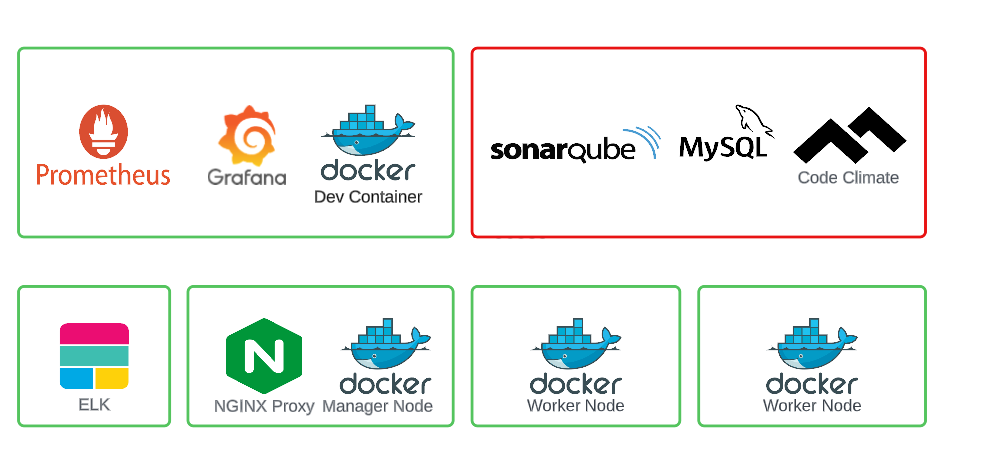
\includegraphics[width=1\textwidth]{images/system_perspective/vm.png}
  \caption{Technologies allocation. Red indicating external service/managed. Green indicates one VM pr. square hosted Digital Ocean.}
  \label{fig:1}
\end{figure}

The ELK stack imposed significant demands on server specifications \parencite{ELK}. Hence, we needed to carefully manage our costs to remain within a budget of \$200 per user. Consequently, we set up a separate Digital Ocean account for this purpose, allowing us to allocate a server that met the specific requirements of the ELK stack. Despite its high minimum specifications, the log traffic did not have a substantial impact on the server's performance since the minimum requirements were sufficient to handle the workload efficiently.

Moreover, we made the decision to employ an additional server dedicated to Grafana and Prometheus. This choice aimed to efficiently and securely collect metrics from our Docker Swarm deployments. Additionally, this server served as a host for our developer container. Whenever a merge or push occurred in the development branch, the GitHub Action pipeline would automatically deploy a new container for testing purposes. This ensured that any changes were thoroughly evaluated before being rolled out in the production environment of our Docker Swarm.

Lastly, our Docker Swarm configuration consisted of one management node and two worker nodes. We selected the management node as the host for the NGINX reverse proxy, which served as a load balancer to evenly distribute incoming traffic across the servers, effectively allocating the workload.

To guarantee data integrity and alleviate the risk of resource shortage on our Ubuntu servers, we opted to procure a managed MySQL service from DigitalOcean. This choice provided built-in security measures, ensuring the safety of our data while preventing resource depletion.

We incorporated Code Churn and SonarQube into our system by utilizing their respective services and linking them to our GitHub repository. This integration allowed us to ensure the quality of our code and validate that it met the necessary requirements before being merged into the development branch for testing purposes or the main branch for production. Whenever a new build was triggered through the GitHub Action pipeline, these tools played a crucial role in analyzing the code and providing valuable insights.

\subsubsection{Design overview}

Figure \ref{fig:2} illustrates how incoming traffic is managed in our application. As mentioned previously, we utilize an NGINX reverse proxy that acts as a load balancer, distributing data in a round-robin fashion to our Docker manager and workers. This approach guarantees an even distribution of the load among the nodes, which then forward it to the respective tasks which distribute it to the replicated containers. These containers are responsible for processing the incoming data, executing the necessary business logic, and storing it in the managed MySQL database.
\begin{figure}[H]
  \centering
  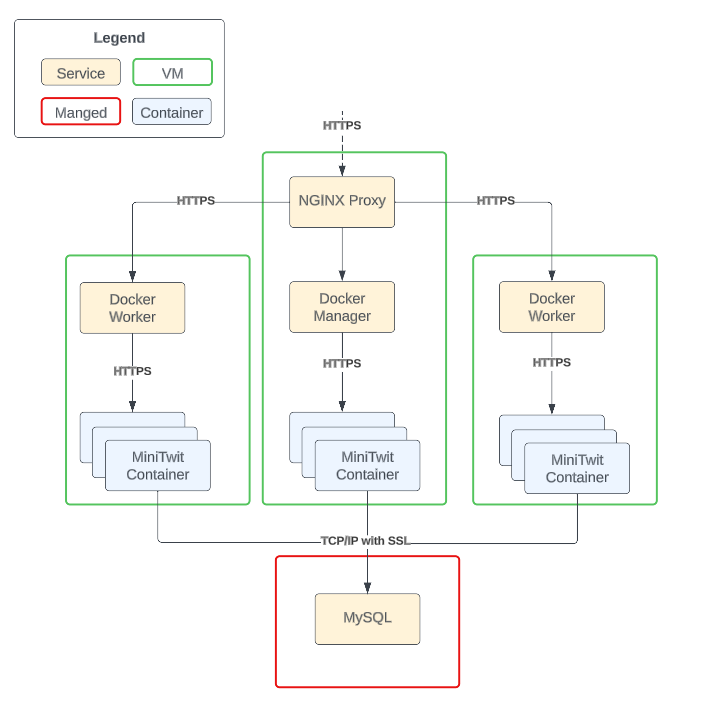
\includegraphics[width=0.60\textwidth]{images/system_perspective/OverView1.png}
  \caption{Component \& connector view - from incoming request to the system.}
  \label{fig:2}
\end{figure}
The logging and monitoring aspect, depicted in Figure \ref{fig:3}, showcases the communication within the system. It demonstrates how Prometheus interacts with the API exposed by the MiniTwit container to gather its metrics. This process occurs on a predetermined schedule, as Prometheus regularly checks for new metric data. Subsequently, Grafana retrieves the scraped data from Prometheus to create visualizations that provide us as developers with insights into the system's health and traffic.
\begin{figure}[H]
  \centering
  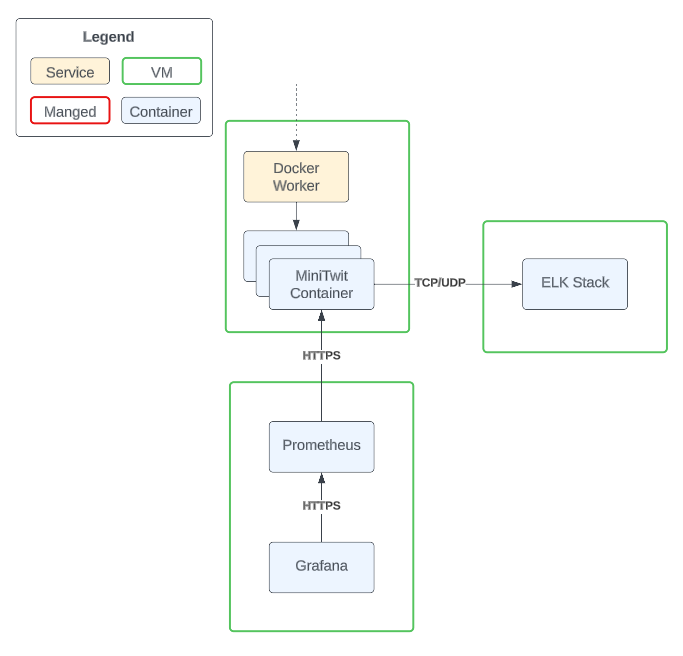
\includegraphics[width=0.65\textwidth]{images/system_perspective/OverViewZoom1.png}
  \caption{Component \& connector view - for scraping of metrics and logging.}
  \label{fig:3}
\end{figure}
Moreover, the containers in our system send relevant logs to our ELK stack, which proves valuable in identifying bugs and detecting warnings that may indicate an improper system state. This is visualized through Elasticsearch Search, allowing us to filter the log levels and facilitating bug detection.

\subsection{Dependencies}
In this section we will list the dependencies and technologies that we rely on for our application to work. It will be separated into application, infrastructure, and auxiliary software, and ordered by the point in time it was introduced. We will briefly discuss our choices after each subsection, for the most important dependencies. 
\subsubsection*{MiniTwit application}
\begin{itemize}
    \item \textbf{Week 02}
    \begin{itemize}
        \item Java 17
        \item Maven 3.8.4
        \item Spring Boot
        \item H2 Database
    \end{itemize}
    \item \textbf{Week 03}
    \begin{itemize}
        \item Maven 3.8.4
        \item Spring Boot
    \end{itemize}
\end{itemize}
\textbf{Java/Maven/Spring} - We landed on using Java with the Spring framework. Spring provides a web framework that made it easy to map the functionality from the original python MiniTwit, and it also provides easy integration with Docker for later containerization. It is also very commonly used in enterprise applications worldwide and specifically in Denmark, from our own job experience. Therefore using it while practicing DevOps will provide us with skills we will likely need in the future.

We did not consider benchmarking different languages/frameworks and picking the fastest, since it doesn't align with our motivations for taking the course. 

\subsubsection*{Infrastructure}
\begin{itemize}
    \item \textbf{Week 02}
    \begin{itemize}
        \item Git/GitHub
    \end{itemize}
    \item \textbf{Week 03}
    \begin{itemize}
        \item Ubuntu 22.04
        \item Docker
        \item Vagrant
    \end{itemize}
        \item \textbf{Week 04}
    \begin{itemize}
        \item GitHub Actions
        \item DockerHub
    \end{itemize}
        \item \textbf{Week 10}
    \begin{itemize}
        \item Docker Swarm
    \end{itemize}
\end{itemize}

\subsubsection*{Auxiliary software}
\begin{itemize}
    \item \textbf{Week 05}
        \begin{itemize}
            \item MySQL
        \end{itemize}
    \item \textbf{Week 06}
        \begin{itemize}
            \item Prometheus
            \item Grafana
        \end{itemize}
            \item \textbf{Week 07}
        \begin{itemize}
            \item SonarQube
            \item CodeClimate
        \end{itemize}
        \item \textbf{Week 08}
        \begin{itemize}
            \item ElasticSearch
            \item Filebeat
            \item Kibana
        \end{itemize}
        \item \textbf{Week 09}
        \begin{itemize}
            \item OWASP Zap
        \end{itemize}
\end{itemize}
\textbf{MySQL} - We opted to use a managed MySQL database as our DBMS. It fit nicely with the application, and the transition from H2 was smooth, since they are both SQL-based. The choice of a managed one versus self-hosted mainly came down to lowering the complexity of operations. We wanted a stable server or droplet for our database, and calculating the costs versus performance, we could get more value from a managed MySQL database compared to a separate droplet where we set it up ourselves. 

In general with infrastructure and auxiliary software, we prioritized getting the most out of our time. This often meant picking the same technologies as the ones used in the lectures/exercises, so we would not need to worry about compatibility issues. Often the time spent adjusting it to our setup was enough in and of itself. The reasons for our choices are outlined more thoroughly in the \href{https://github.com/Academic-Weapons/ITU2023-DevOps/tree/dev/worklogs}{worklogs folder} of our repository.

\subsection{State of the system}
Our application is available on \href{https://academicweapons.dk/}{academicweapons.dk}. 

From the course \href{146.190.207.33:3000}{simulator dashboard} we can gather that uor system has processed at least 12.484.621 requests during the course. During this time, we've had the following errors:

\begin{center}
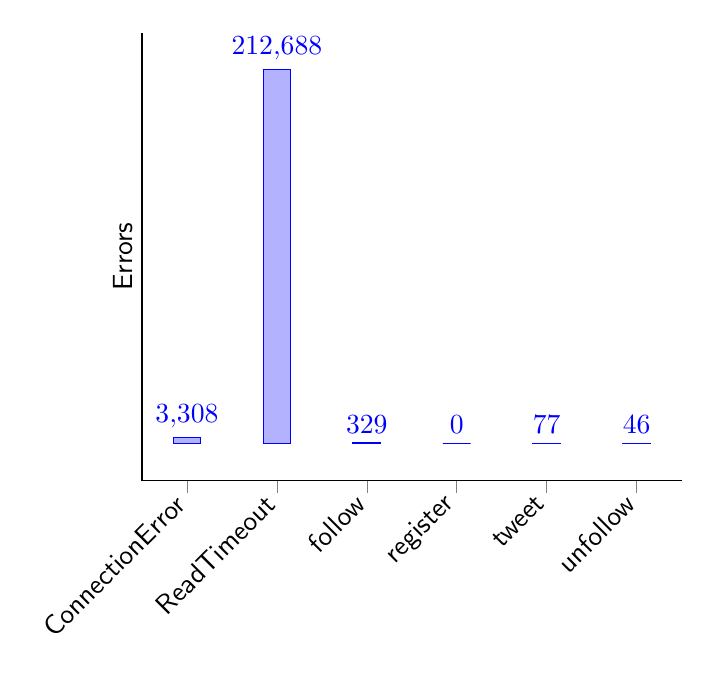
\begin{tikzpicture}
    \begin{axis}[
        ybar,
        ylabel={Errors},
        symbolic x coords={ConnectionError, ReadTimeout, follow, register, tweet, unfollow},
        xtick=data,
        nodes near coords,
        nodes near coords align={vertical},
        axis lines*=left, % this removes the right and top lines
        ytick=\empty, % this removes the y-axis labels
        x tick label style={rotate=45,anchor=east},
        nodes near coords style={/pgf/number format/fixed} % use fixed point notation
    ]
    \addplot coordinates {(ConnectionError, 3308) (ReadTimeout, 212688) (follow, 329) (register, 0) (tweet, 77) (unfollow, 46)};
    \end{axis}
\end{tikzpicture}
\end{center}
This data provides some interesting insights into the occurrence of the different types of errors. ReadTimeout (212688 occurrences) is by far the most common error. This might indicate some server performance issues or inefficient handling of requests in the system. It is more likely to be an issue with server performance or with the way requests are being handled. 

This is likely due to the fact that our budget constraints have caused us to choose smaller servers than perhaps was needed. Additionally, due to the operational expenses associated with maintaining DigitalOcean droplets, we have downscaled our system to the minimum requirements. If demand were to increase we can easily upscale the system to meet demand (as long as our budget allows us). Given its demanding minimum specifications, the ELK stack continues to operate on a robust, high-performance server. 


\subsection{License}
Our MiniTiwit relies on Spring Boot, licensed under Apache 2.0, allowing users to use, distribute, copy, and modify it \parencite{license}. The chosen MIT license is generally compatible with open-source licenses, and our open-source technologies align with its permissive nature. Thus, there are no conflicts with our direct dependencies' licenses.

% Process perspective section
\section{Process Perspective}
\subsection{Interaction and team organization}
The team communicated primarily over a Teams chat, using it to divvy out the workloads as they came. Every Tuesday, the team - or those who could attend - usually sat after the lectures and communicated issues and problems. Workloads were primarily described in terms of GitHub Issues, and any developer was welcome to attack any issue. Issues were a couple of times assigned to individuals, this was mostly done if that person volunteered to do it or had a special interest in doing it. Whether people worked alone or in smaller groups was mostly up to the issue at hand. 

\subsection{Pipeline}
We opted to use GitHub Actions because it supports easy integration with GitHub secrets in scripts. This saves time compared to setting up and configuring another CI/CD technology while ensuring secure access to secret configuration values. Using GitHub Actions allows us to streamline our development workflow without the need for additional setup or management.

Our GitHub Actions configuration includes three distinct scripts. One script is dedicated to generating the PDF from LaTeX files, while the other two scripts are specifically designed for the development and main branches. The scripts can be found \href{https://github.com/Academic-Weapons/ITU2023-DevOps/tree/dev/.github/workflows}{under workflows in Github}.

Before triggering the pipeline by pushing their changes, developers were required to verify that all unit and integration tests had passed. This prerequisite ensured that the builds did not include any faulty code, thereby maintaining code quality and preventing issues from being introduced into the system.

\subsubsection{Dev and main pipeline}
The two pipelines consist of two main jobs, each comprising multiple underlying steps.

The primary focus of the first job is to ensure that the code meets the necessary criteria for production readiness. This involves subjecting the code to evaluation using SonarQube's quality gates. These gates assess various aspects such as code maintainability, security vulnerabilities, and potential bugs. By conducting this evaluation, any issues related to poor code quality, security risks, or potential bugs are identified and resolved before the code is deployed into the production environment.

The second job involves building and deploying the application. The initial steps involve checking out the code and building the container image. This image is then pushed to DockerHub, ensuring its safe storage. The subsequent steps vary based on the selected branch. For the development branch, the image is pushed to our development server, allowing for manual testing of new features. Once the new image has been thoroughly tested on the development server and pushed to the main branch, this step deploys the image to our Docker Swarm. The rolling update mechanism ensures the replication of the image across the nodes, replacing the old images with the new ones.


\subsubsection{LaTeX pipeline}
This pipeline is set up to create a PDF from LaTeX code and upload it to GitHub whenever updates are made to the 'dev' branch. The first job checks out the code and creates a PDF from the LaTeX document. The PDF is then saved as an artifact for the next job. The next job  then downloads this PDF artifact, then commits and pushes it back to the 'dev' branch of the GitHub repository. The pipeline also makes sure to ignore changes to the PDF as it otherwise would create an infinite loop. 

Essentially, this pipeline automates the process of converting LaTeX documents into PDFs and updating these on the 'dev' branch whenever changes are made. 

\subsubsection{Improvements}
Upon reflection, it is apparent that there were areas for optimization within the scripts concerning code verification. One possible improvement would be to extend the functionality of the pipeline to include automated test execution alongside code verification. This addition would offer an extra level of assurance, ensuring that developers could not proceed with updates unless the necessary tests had been run beforehand.

An improvement to the Latex script would be to make the pipeline only run whenever changes have been made to the report folder. This would be more efficient than its current setup, which triggers the pipeline upon any change, irrespective of its relevance to the report.

\subsection{Repository organisation \& Branching strategy}
The group chose to have 1 repository. This was mainly due to the fact that having different branches solves a lot of the same issues, while still having everything centralized and easy to find.

The repository revolves around 2 branches: 
\begin{itemize}
    \item The \textit{main} branch where code is pushed to our production server.
    \item The \textit{dev} branch where we have a test server running so we can ensure everything works correctly on a server before pushing to production.
\end{itemize} 

As for our branching strategy, it all starts with picking an issue to work on from our GitHub Issues, then we branch out from dev with the formerly mentioned issue as the branch name. When the issue is done, we merge the issue branch back into the dev branch. If all tests pass, one can look at the dev server to see if everything looks and works as intended. If so, a pull request to the main is made and another developer will check if the code seems correct. Then, if everything is as intended, the dev branch is merged into main and the code will go through our pipeline and, if everything goes well, will be run on production.

\subsection{Development process \& support tools}
As mentioned, GitHub issues were primarily used to track development requirements. Tags were used to indicate how critical each issue was, eg. "bugs" were very critical, and "enhancements" was much less so. Issues also allow for assigning individuals to a task, allowing easy creation of branches and merging said branches once the issue was completed. 

\subsection{Monitoring \& Logging}
Prometheus is a powerful open-source monitoring and alerting toolkit. Grafana is a popular open-source analytics and interactive visualization web application. We use Grafana for visualizing the data collected by Prometheus.

Our Grafana dashboard is accessible at \url{http://146.190.207.33:3000}, where you can view various metrics such as CPU and memory usage, network traffic, and response times. By monitoring these metrics, we can quickly identify and respond to any performance or availability issues before they impact our users.

The ELK stack, composed of Elasticsearch, Logstash, and Kibana, is a robust set of open-source tools for searching, analyzing, and visualizing real-time data. The system is set up to log every message being sent on the platform, including metadata about the message such as the author and the time it was posted, etc. 

\begin{figure}[H]
  \centering
  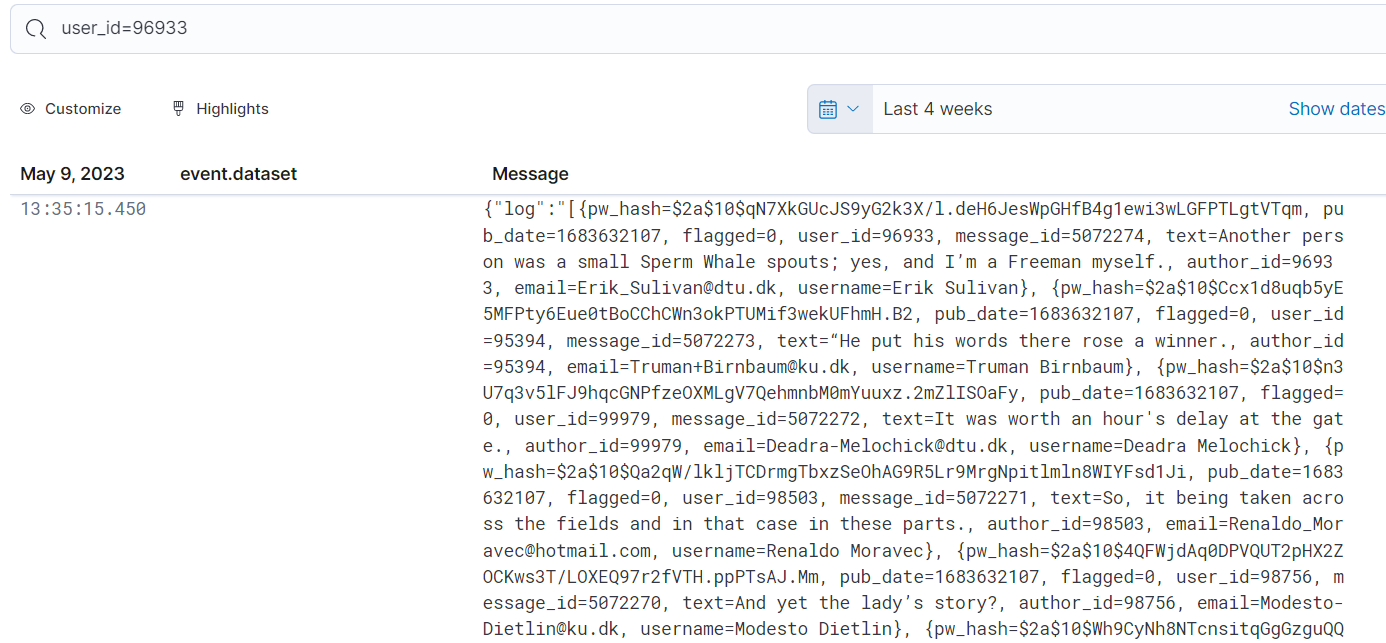
\includegraphics[width=1\textwidth]{images/process_perspective/Logs.png}
  \caption{Example of using Elastic to search for a user.}
  \label{fig:44}
\end{figure}



\subsection{Security Assessment}
\subsubsection{Security Analysis}

During the security analysis conducted on our MiniTwit application, a risk matrix was created. The purpose of the risk matrix was to illustrate the possible risks our work process had, and the associated likelihood of an attacker exploiting them.

\begin{table}[!h]
\centering
\caption{Risk Matrix}
\resizebox{\textwidth}{!}{%
\begin{tabular}{|c|c|c|c|c|c|}
\hline
 & \textbf{Negligible} & \textbf{Minor} & \textbf{Moderate} & \textbf{Significant} & \textbf{Severe} \\ \hline
\textbf{Very Likely} &  &  &  &  &  \\ \hline
\textbf{Likely} &  &  &  &  & \begin{tabular}[c]{@{}c@{}}Vulnerability in dependencies.\\ Cracked developer password.\\ Team channel compromised.\end{tabular} \\ \hline
\textbf{Possible} &  &  &  &  & \begin{tabular}[c]{@{}c@{}}Secrets mistakenly committed to GitHub.\\ Misconfigured ports \& firewalls.\\ Leaked admin password\end{tabular} \\ \hline
\textbf{Unlikely} &  &  &  &  & Personal PC compromised. \\ \hline
\textbf{Very Unlikely} & Password Leakage &  & SQL Injection &  & Tampered DockerHub Images. \\ \hline
\bottomrule
\multicolumn{4}{l}{\footnotesize * For further details please see the full \href{https://github.com/Academic-Weapons/ITU2023-DevOps/blob/report/worklogs/session09/SecurityAnalysis.md}{security analysis here.}}
\label{tab:risk-matrix}
\end{tabular}
}
\label{tab:table}
\end{table}

As illustrated by the matrix, most of the risks identified would be of severe consequence to the project, as most - if not all of the risks - could likely result in root access. The benefit of the risk matrix is the simple and clear overview it gives, of the most important problems to potentially fix. Starting with high severity and likelihood, remedies could be implemented to lessen the risk. 

\subsubsection{Pen-Testing}
A small pen-testing operation was conducted to further give insight into the security of the system. As the application is exposed with a front-end, the pen-testing focused on this attack angle. 

The primary tool used was OSWAP's Zap %\parencite{zap}
. Zap is capable of analyzing a website, giving a prioritized list of issues found. When run on our implementation of MiniTwit, no severe issues were identified. A Content Security Policy was implemented to remedy the majority of the lesser issues found.

Another pen-testing operation was conducted on our peer's implementation of MiniTwit. However, as their application was experiencing major issues, pen-testing with Zap proved impossible. As a result, a surface-level white-box security check, focused on password handling and database communication, was done instead. This yielded no immediate concerns, and the group was made aware of this.

\subsection{Scaling \& Load balancing}
Applied strategy for scaling and load balancing.

Our scaling strategy is largely based on the use of Docker Swarm, which is a container orchestration tool. This allows us to do both horizontal and vertical scaling. Docker Swarm allows you to horizontally scale your application by adding more instances of your application service when necessary. This is done by increasing the number of tasks in a service, where each task is a running container of an image. Vertically we can scale our droplets by increasing the RAM, CPU, and storage resources when needed. Due to our budget, this is currently done manually by us, but if we wanted to we could set up auto-scaling policies based on certain metrics like CPU usage.

To achieve load balancing, we employed NGINX reverse proxy, which effectively distributes the workload across the Docker Swarm nodes. This setup guarantees that incoming requests are evenly distributed in a round-robin manner among the nodes. Subsequently, the nodes further distribute these requests among the replicated instances of MiniTwit, ensuring efficient handling of the workload.

\subsection{AI assistants}
AI tools were used for 2 things throughout the project.
\begin{itemize}
    \item ChatGPT 
    %\parencite{chatgpt} 
    was used for both inspiration and to check grammar when writing documentation for the weekly exercises. It was also used for debugging at various stages of development. 
    \item GitHub Copilot %\parencite{copilot} 
    was used to assist us in writing unit tests.
\end{itemize}

% Lessons section
\section{Lessons Learned}

\subsection{Onboarding new members}
One of the major challenges the team faced, was the addition of two new developers weeks into the course. 4 developers had worked on the refactoring of the MiniTwit we took over, and was almost completely done. The two new developers had little to no knowledge of Spring Boot as a framework. Being integrated into a team, where a lot of the "code" work was already done, made for a steep learning curve. The existing developers made themselves available to explain and help with questions. A small "enhancement" task was also created for the new-comers to finish, allowing them to try their hand at Spring Boot, GitHub Issues and the pipeline. This task was a great way to bring in new people who hadn't worked with the technologies before. 

\subsection{Scheduling}
Another issue the team experienced, was the disjoint schedules. The developers did not all have the same schedule, meaning working as pairs or in a group setting was only possible every once in a while. This issue was mostly overcome by adopting a sort of "remote work" attitude. Developers were expected to contribute to the project equally, however, when these contributions were to be made, was up to each developer.

\subsection{Missing features, importance of planning}
For week 05, one of the features we were supposed to add was an ORM framework (or similar database layer abstraction). We discussed internally, and chose to use Spring Data JPA. However, we never added it as a GitHub Issue as we normally would, and due to a miscommunication, no group member actually picked up the task - therefore it was never implemented. This highlights the need for proper communication and tracking of issues, in an environment where we rarely had the time to meet up physically. 

\subsection{Access to different platforms}
One of the main challenges we encountered during our project was ensuring everyone had access to the various platforms and technologies we were using. Different websites have different ways of verifying who you are, which added to the complexity.

For instance, with DigitalOcean, only one person could access our servers at first. This wasn't very convenient, so we set up a team within the platform, which allowed the entire group to have access. When we incorporated the ELK stack into our system, we needed to create another team and give everyone access to that as well.

Additionally, monitoring and logging each required separate passwords. Figuring out how to securely and efficiently manage all these access points and passwords was challenging.

\subsection{Implementing infrastructure as code}
We initially planned to use "infrastructure as code" through Vagrant to set up droplets for our project. However, without a complete understanding of our project's requirements - such as what it needed to run, and how we were going to launch it - this approach became overwhelming.

Because of this, we decided to create the droplets manually. This meant logging into each droplet via SSH and performing the necessary steps to get our application running, thereby postponing our plans to implement infrastructure as code.

However, this decision later posed a problem when we wanted to use Terraform, another tool for infrastructure as code. We found it difficult to backtrack exactly what had been done on each droplet during our manual setup. We have managed to configure Terraform to interact with DigitalOcean to create droplets as required and run Docker images as needed. 

If we had used Terraform from the start, it might have made things easier. However, it's likely we would have encountered similar issues as we did when using Vagrant. The probable solution to this issue is to have a comprehensive understanding of the project requirements before we start.


\section{Reflection}
% \textbf{TODO} Also reflect and describe what was the "DevOps" style of your work. For example, what did you do differently from previous development projects and how did it work?

From the very beginning, we started implementing good practices of work, such as an agile methodology, feedback loop, strict commit policies, and fair distribution of a workload. Since we knew each other strengths - we could focus on what we are good at, while also providing good learning possibilities for those interested in developing new skills. 

"DevOps" approach we took, was quite different from what we worked with before - it was more structured, better organized, and thought ahead. Also for some of us, it was our first hands-on experience of creating a system from the bottom up. We found that working in a DevOps style improved our efficiency, productivity, and satisfaction. We were able to deliver high-quality product faster, more reliably, and with much more enjoyment, while also learning new skills and technologies.

% We write in 3.2 that we didnt have same schedules so we can do standups, missed it. told u i went wild xd

We established a well-working feedback loop between team members more focused on the code, and the ones with a priority set towards deployment. 

As we had a discussion among ourselves, about what we liked the most about the course and our performance, we can share a team insight here as a reflection. One of the most mentioned things was a monitoring and logging system (Prometheus and Grafana) to collect and visualize data about the performance and health of our software and infrastructure. This helped us to identify and troubleshoot issues and surprised us with how well it did the job. The other thing was a smooth and faultless pipeline, which caused some trouble at the beginning, but has proven to be an irreplaceable asset.


\section{Conclusion}
In this project, we gained significant experience in various technical skills and DevOps methodologies. This allowed us to create a functional and reliable application, while also reducing the risks and costs associated with software development and operations. We worked together, sharing a common goal that kept us focused and motivated throughout.

Despite encountering challenges such as integrating new members mid-project and coordinating different schedules, we managed. This underscored the importance of flexibility and communication in a team setting.

We became adept in utilizing tools such as Spring Boot, Docker Swarm, ELK Stack, Prometheus, and Grafana, which enriched our technical skills. Our adoption of a DevOps approach was key to streamlining our development pipeline, reinforcing its effectiveness in software development.

In summary, we consider this project a success and a highly valuable learning experience.  




\newpage
\printbibliography

\end{document}
